\chapter{Implementation} \label{chap:implementation}

We approach the problem of spectral uplifting similarly to~\citet{upsamplingJakobHanika}, where an uplifting model is created prior to rendering. Our implementation therefore consists of two parts --- \emph{model creation} and its subsequent \emph{utilization} in a rendering software. 

For the first part, we extend an already existing uplifting tool, the \emph{Borgtool}, which is currently used for creating sigmoid-based RGB cubes in the same manner as in~\cref{alg:upliftingAlgSigmoid}. We add the possibility for creating trigonometric moment-based cubes (from now on referred to as \emph{trigonometric moment cube}), i.e. for the spectra to be stored with trigonometric moments rather than sigmoid coefficients. We also add an option for constraining such a cube with a user-specified atlas.

We then show the performance of such a model by integrating it in ART, which, up until now, used only one built-in sigmoid-based cube for all its uplifting processes.

\section{Uplifting model}

The core of this section is the already mentioned Borgtool. It is a stand-alone, non-open source thing that was created by Weta and is .

The output of the Borgtool is an RGB cube structure which contains multiple entries in form of lattice points. Following, we name the main parameters of a single cube entry of the already supported sigmoid-based cube:
\begin{itemize}
	\item \emph{target RGB} --- the RGB coordinates that the point has in the cube
	\item \emph{coefficients} --- 3 sigmoid coefficients used to reconstruct a spectrum so it matches the target RGB
	\item \emph{lattice RGB} --- the actual RGB that the reconstructed spectrum evaluates to. Ideally, this should match the target RGB
\end{itemize}
Along with its entries, the resulting cube structure also stores a few other properties, both \emph{static}, such as the illuminant according to which the RGB cube is uplifted, and \emph{user-adjustable}, such as the cube dimension or the fitting threshold (i.e. the maximum allowed difference between the target and the lattice RGB).

Our trigonometric moment cube can be viewed as an extension of the sigmoid cube, as it keeps most of its parameters and mainly extends the already existing ones. The main difference between them lies in the distinction of the lattice points --- while the sigmoid cube regards all of its points as equal, the trigonometric moment cube distinguishes (by means of a \texttt{seeded} boolean parameter) between \emph{atlas lattice points}, i.e. the lattice points that store the user-inputted RGB:spectra mappings; and \emph{regular points}, which do not.

Our requirements for the shape of the spectra at atlas lattice points differ from the ones at regular lattice points. While we prefer the regular lattice points to have their spectra as smooth as possible in order to avoid unexpected artifacts under other illuminants, the coefficients of the atlas lattice points must reconstruct spectra almost identical to the input spectra, which might include sharp edges and spikes.

Therefore, it is sufficient for the regular lattice points to be represented with a smaller number of coefficients, while atlas lattice points might require a lot more. Although a smooth spectrum can be represented with a high number of coefficients, such a representation is memory inefficient, its reconstruction is more time consuming, and, most importantly, it does not work well with the optimizer. Based on our experiments in~\cref{ssec:noOfMoments}, we decide to store the spectra of regular lattice points with 3 coefficients and adjust the number of coefficients of the atlas lattice points depending on the nature of its desired spectrum.

In addition to supporting variable number of coefficients (ranging from 3 to 24), the trigonometric moment cube also supports the possibility of a multiple coefficient representations per lattice point. The sole purpose of such extension is to lower the cube size requirements upon constraining, which we address more thoroughly in ref.

In addition to the cube structure, the uplifting process of the trigonometric moment cube is also similar to the one of the sigmoid cube, which closely follows~\cref{alg:upliftingAlgSigmoid}. Its main distinctions are in the constraining process (which the sigmoid cube lacks) and in the first round of fitting.

Following, we name the individual steps of the process, which we then analyze in greater detail.
\begin{enumerate}
	\item \emph{Initialization}
	\item \emph{Cube seeding (optional)}
	\item \emph{Fitting of starting points}
	\item \emph{Cube fitting}
	\item \emph{Cube improvement}
	\item \emph{Cube storage}
\end{enumerate}

\subsection{Initialization} \label{ssec:initialization}

This part of the run is responsible for three things:
\begin{itemize}
	\item parsing of the parameters
	\item initialization of the cube and its entries with default values
	\item loading of the required color atlases
\end{itemize}

The initialization of the cube is pretty straightforward, as all of its properties are either user-defined or set to default (note: the default illuminant is always D65). The number of cube entries is directly proportional to the cube's \texttt{dimension} parameter, which specifies the number of entries per one axis. This renders the total number of entries to $dimension^3$. As the lattice points are positioned evenly, their target RGB values are equivalent to their coordinates in the RGB cube.

The loading of the atlases is a bit more complicated. Firstly, a single color atlas is inputted in a form of a simple .txt file, which contains merely a list of entries in a textual form as shown in~\cref{fig:macbethSampleText}. Therefore, it requires parsing.

\begin{figure}
	\lstset{
		string=[s]{"}{"},
		comment=[l]{:},
		commentstyle=\color{black},
		basicstyle=\scriptsize
	}
	\begin{lstlisting}[label=lst:atlasEntry]
	Entry ID:   orange
	------------------------------------------------------------------------
	Description           :  "orange" patch of the Macbeth colour checker
	Type                  :  reflectance spectrum
	Fluorescence data     :  no
	Measurement device    :  
	Measured by           :  
	Measurement date      :  
	
	Sampling information
	--------------------
	Type	    	      :  regular
	Start                 :  380.0 nm
	Increment             :  5.0 nm
	Maximum sample value  :  100.0
	
	ASCII sample data
	-----------------
	{6.143748,  5.192119,  4.867970,  5.092529,  4.717562,  4.663087, 
	4.455331,  4.562958,  4.517197,  4.536289,
	4.454180,  4.543101,  4.491708, ... }
	\end{lstlisting}
	\caption{A sample entry from the Macbeth Color Checker atlas}
	\label{fig:macbethSampleText}
\end{figure}

Moreover, the spectral data obtained from the atlases cannot be stored in the Borgtool directly, so as to avoid extreme memory requirements arising with large atlases. To solve this problem, we take advantage of the trigonometric moments.

We store the spectral curves of the individual atlas entries with Fourier coefficients as described in~\cref{par:spectrumToCoefficientConversion}. We mirror but do not warp the signal prior to coefficient computation (see~\cref{sec:storingMoments}).

The number of coefficients per atlas entry is variable, ranging from 4 to 24. We explain our method for determining the sufficiency of coefficient representation, and therefore the coefficient count for each atlas entry, in~\cref{ssec:noOfMoments}.

\subsection{Cube seeding} 

In order to uplift the whole cube as described in~\cref{alg:upliftingAlgSigmoid}, we must first fit one or more \emph{starting points}, whose coefficients can then be used as prior for the fitting of other lattice points. For these purposes, we utilize the user-specified color atlas. The general idea behind this process is to copy the coefficients of atlas entries to specific lattice points, and then use these coefficients as prior for fitting said lattice points. We refer to this process as \emph{seeding}, and term the seeded lattice points \emph{atlas lattice points}.

The ideal scenario would be if the RGB of the atlas entries were to perfectly match the coordinates of lattice points. However, as the RGB value of an atlas entry can be virtually any triplet within the (0,1) range, it is most likely that the atlas entries evaluate to a point inside the cube voxel.

A realistic approach would be to create a complete injective mapping between the atlas entries and their closest lattice points. However, such a mapping would provide satisfactory results only if we were to use the nearest-neighbor method for uplifting non-mapped RGB triplets. If we were to use either the interpolation of coefficients or spectra, which both employ all 8 voxel corners during the uplift, the curves of uplifted RGB values of atlas entries would most likely be considerably distinct from the desired result (i.e. the original atlas entry spectrum), subsequently causing color artifacts. We can observe this behavior in~\cref{fig:seedingMethod1corner}. However, as seen in~\cref{fig:seedingMethod8corners}, propagating the information about the original reflectance of the entry to all voxel corners improves the result remarkably. We therefore opt for seeding all 8 voxel corners per an atlas entry.

\begin{figure}[t]
	\centering
	\begin{subfigure}[t]{0.54\textwidth}
		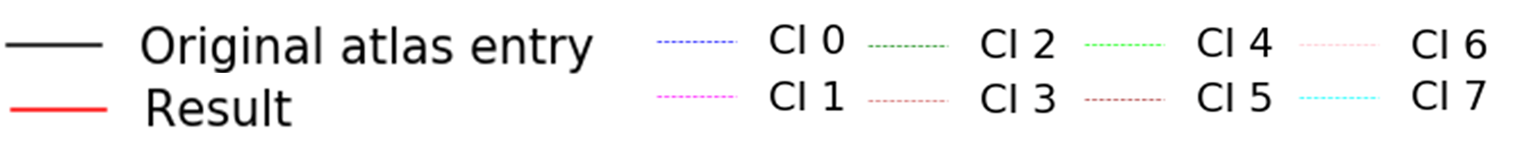
\includegraphics[width=\linewidth]{img/seeding_method_legend.png}
	\end{subfigure} \\
	\begin{subfigure}[t]{0.45\textwidth}
		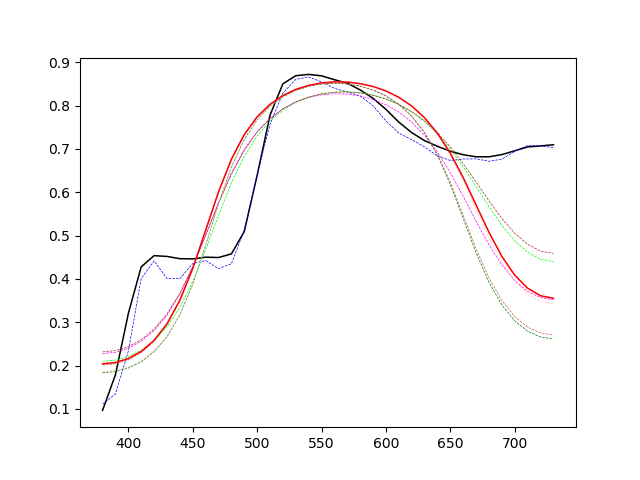
\includegraphics[width=\linewidth,height=0.2\textheight]{img/seeding_method_1corner.png}
		\caption{Only 1 voxel corner seeded}
		\label{fig:seedingMethod1corner}
	\end{subfigure} \hspace{0.1em}
	\begin{subfigure}[t]{0.45\textwidth}
		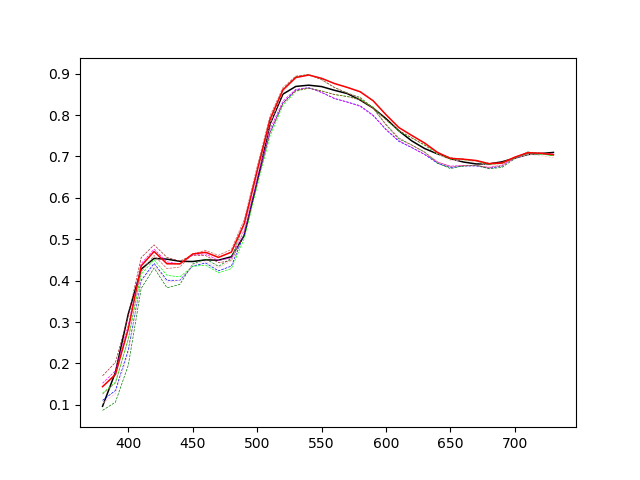
\includegraphics[width=\linewidth]{img/seeding_method_8corners.png}
		\caption{All 8 voxel corners seeded}
		\label{fig:seedingMethod8corners}
	\end{subfigure}
	\caption{Comparison of the performance of two seeding methods}
	\label{fig:seedingMethodInterpolation}
\end{figure}

During the seeding process, it may occur that two atlas entries would fall into neighboring voxels, i.e. that they would share some of the voxel corners. We solve such collisions by utilizing the possibility of one lattice point having multiple coefficient representations. In addition to coefficients and their count, we also store an entry ID per each representation, so as to later distinguish the reconstructed curves during rendering and decide which to employ, which we explain in more detail in ref.

If two atlas entries fall into the same voxel, however, there is no way to determine the interpolation of which the user desires upon uplifting the RGB values inside said voxel. We therefore discard one of the entries and throw an error informing the user of the collision and suggesting to increase of the cube dimension.

We show an example of a cube seeded and subsequently fitted with the Munsell Book of Colour in~\cref{fig:seededCubeMCB}. Lattice points marked as black represent the seeded points. Note that a lot of these points store multiple coefficient representations.

\begin{figure}[t!]
	\centering
	\captionsetup[subfigure]{font=footnotesize,labelfont=footnotesize}
	\captionsetup[subfigure]{justification=centering}
	\begin{subfigure}[t]{0.22\textwidth}
		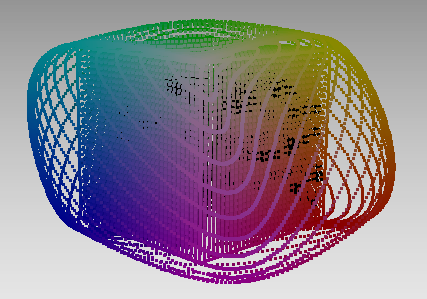
\includegraphics[width=\linewidth]{img/seededCube_mcb1.png}
		\label{fig:seededCube_mcb1}
	\end{subfigure} \hspace{0.05em}
	\begin{subfigure}[t]{0.22\textwidth}
		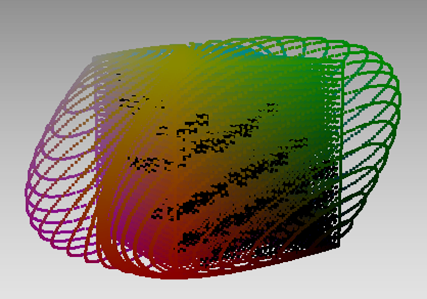
\includegraphics[width=\linewidth]{img/seededCube_mcb2.png}
		\label{fig:seededCube_mcb2}
	\end{subfigure} \hspace{0.05em}
	\begin{subfigure}[t]{0.22\textwidth}
		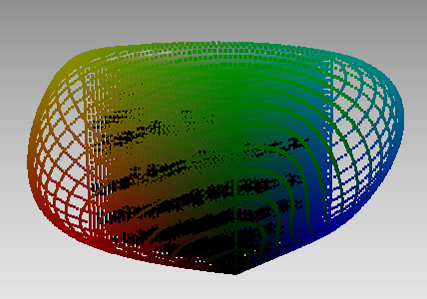
\includegraphics[width=\linewidth]{img/seededCube_mcb3.png}
		\label{fig:seededCube_mcb3}
	\end{subfigure} \hspace{0.05em}
	\begin{subfigure}[t]{0.22\textwidth}
		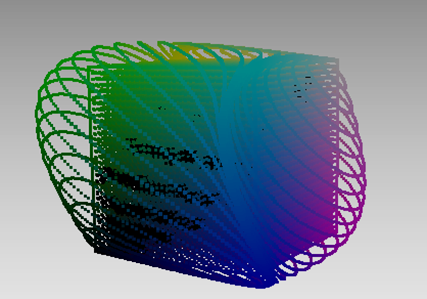
\includegraphics[width=\linewidth]{img/seededCube_mcb4.png}
		\label{fig:seededCube_mcb4}
	\end{subfigure}
	\caption{A 32-dimensional cube fitted with the Munsell Book of Colour}
	\label{fig:seededCubeMCB}
\end{figure}

Constraining the uplifting process with an atlas is optional. If no atlas is inputted, all lattice points are regarded as regular lattice points and the cube is fitted from the middle in the same manner as the sigmoid cube. However, the resulting uplifting structure provides no advantages over the sigmoid cube.

We provide a comparison between the starting points when seeding from the middle (either with our or the sigmoid method) and when seeding with an atlas in~\cref{fig:seededStartingPoints}, so as to have a rough idea of their placement.

\begin{figure}[t]
	\centering
	\captionsetup[subfigure]{font=footnotesize,labelfont=footnotesize}
	\captionsetup[subfigure]{justification=centering}
	\begin{subfigure}[t]{0.45\textwidth}
		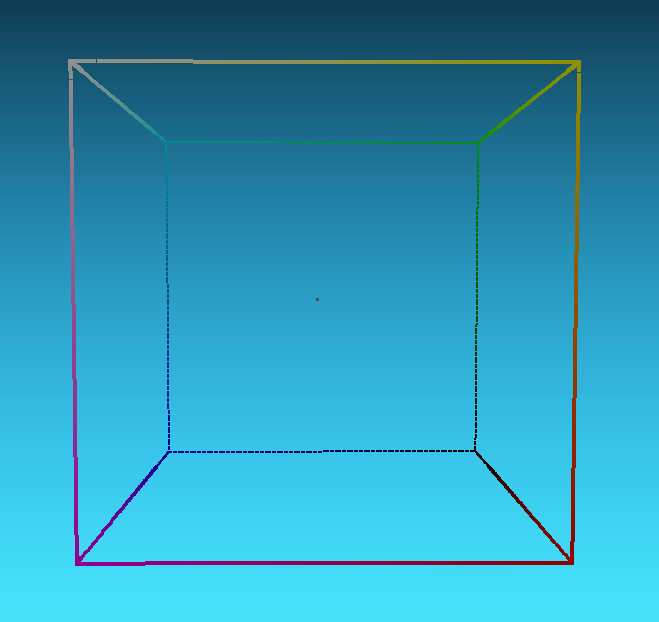
\includegraphics[width=\linewidth]{img/seededStarting_sigmoid.png}
		\label{fig:seededStarting_sigmoid}
	\end{subfigure} \hspace{0.2em}
	\begin{subfigure}[t]{0.45\textwidth}
		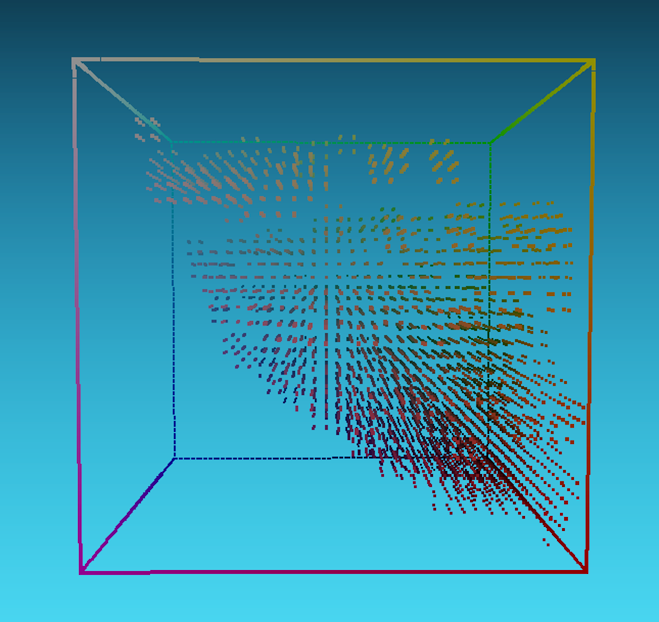
\includegraphics[width=\linewidth]{img/seededStarting_mcb.png}
		\label{fig:seededStarting_mcb}
	\end{subfigure}
	\caption{Comparison of the placement of starting points when seeding with the Munsell Book of Colour (right) and when fitting from the middle with sigmoids (left)}
	\label{fig:seededStartingPoints}
\end{figure}

\subsection{Fitting of starting points} \label{ssec:startingPointsFitting}

By seeding the cube, we have appointed coefficients to some of the lattice points. These coefficients reconstruct a spectrum that evaluates to an RGB value which we denote as the \emph{lattice RGB}. The difference between the lattice and the target RGB is therefore equal to the distance between the lattice point and its assigned atlas entry in the cube. It is apparent that the distance may be higher than the defined fitting threshold. In such cases, we must ``improve'' upon the coefficients so that the resulting color difference is as low as possible.

Our problem of improving the coefficients satisfies the definition of the \emph{Non-linear Least Squares} problem~\cite{nonLinearLeastSquares}. Non-linear Least Squares is an unconstrained minimization problem in the following form:
\begin{equation} \label{eq:nonLinearLeastSquares}
	 \underset{x}{\text{minimize}} \hspace{0.5em} f(x) = \sum_{i} f_{i}(x)^{2},
\end{equation}
where $x= \{x_{0}, x_{1}, x_{2}, ... \}$ is a parameter block that we are trying to improve (i.e. our coefficients) and $f_{i}$ are so-called \emph{cost functions}. The definition of cost functions is dependant solely on the current problem. In our case, we primarily require to minimize the difference between the lattice and the target RGB. Our secondary requirement is for the shapes of the original atlas entry curve and the reflectance curve of the atlas lattice point to be similar. This gives rise to multiple choices for cost functions, such as using the difference between curves along with the Delta E error, using one or multiple cost functions for the RGB error etc\ldots After implementing some of them and testing their performance, the results of which we provide in~\cref{ssec:costFunctions}, we decided on using four cost functions --- three for specifying the absolute difference in one of the three axes of the cube, and one for specifying the average distance between curves per wavelength sample.

To solve an optimization problem defined in the way as described above, we use the CERES solver.

\subsubsection{CERES solver} \label{sssec:ceresSolver}

As already mentioned in~\cref{sec:upliftingMethods}, the CERES solver is an open-source library for solving large optimization problems such as our Non-linear Least Squares problem. It consists of two parts --- a \emph{modeling API} which provides tools for the construction of optimization problems, allowing us to set parameters such as maximum number of iterations of the optimizer or maximum number of consecutive nonmononotic steps; and a \emph{solver API} that controls the minimization algorithm.

To solve a Non-linear Least Squares problem, the solver requires us to specify only a so-called \emph{residual block}, which is a structure defined by the prior coefficients and the cost functions. During the execution, the solver attempts to minimize the values of the cost functions (or \emph{residuals}) in the residual block. The execution is aborted and the current best parameter block returned when the solver achieves either the specified number of iterations or nonmonotonic steps. For more information on the specifics of the CERES solver, we refer the interested reader to its documentation by~\citet{ceresNonLinearLeastSquares}.

There is one main downsides to using the CERES solver. As it is designed to handle very large, sparse problems where every residual term depends on only a few of the input parameters, it is not ideal for solving problems with only one large parameter block. If it is presented with such a problem, its likelihood of getting stuck in local minima and therefore producing unsatisfactory results increases. 

As the atlas lattice points occasionally need to have a rather high number of seemingly unrelated coefficients as parameters, it falls into this category.

Therefore, the more coefficients we use for the representation of atlas lattice point, the more likely we are to encounter the optimizer's failure.


In such cases, the optimizer is not capable of leaving the local minima on its own. We therefore apply a simple heuristics, which consists of only slightly altering the first coefficient (or the first and the second) and running the optimizer again. We chose to alter the first coefficients because they influence the shape of the curve the most.

The need for a heuristic suggests considerable difference between the prior and the resulting coefficients, which implies distinct spectral curves. Such a behavior is undesired, as it may result in strong metameric artifacts. Fortunately, this heuristic is rarely triggered. We examine this in ref, where we analyze the success rate of the fitting and also demonstrate the curve differences by showing both the spectral curves of the atlas entries and of the fitted lattice points.

The sigmoid-based method approaches the starting points problem by selecting the point in the center of the cube and initializing its coefficients to zero. As these values are extremely close to the real values of coefficients, the optimizer does not have a problem with the fitting.

We inspire ourselves by this approach and provide an option for starting in the middle as well. This eliminates the obligation of the user to specify an atlas, i.e. if no atlas is specified, the cube is fitted from the center. However, providing such an option requires us to define a set of prior coefficients for the center point. We determine it by iterating over multiple existing color atlases and searching for spectral curves that roughly evaluate to an RGB of $(0.5, 0.5, 0.5)$. The coefficients of such curves are roughly $\{0.5, 0, 0, 0, ... \}$, i.e. all zeroes except for the first coefficient. We use these prior coefficients for all available moments and cube dimensions.

\subsection{Cube fitting} \label{ssec:cubeFitting}
Once the starting points are successfully fitted, we can use their coefficients as prior for other lattice points. We proceed similarly to the approach in~\cref{alg:upliftingAlgSigmoid}, where the lattice points are fitted in multiple \emph{fitting rounds}, each round attempting to fit the neighbors of the already fitted points. We provide a more detailed description of the principle behind our fitting algorithm in~\cref{alg:upliftingAlgMoments}.

\begin{algorithm}[t!]
	\caption{Fitting of the cube from starting points}
	\label{alg:upliftingAlgMoments}
	\begin{algorithmic}[1]
		\State $n \gets $ user-defined number of coefficients
		\State $fittingRound \gets$ $0$
		\State $unfittedPoints \gets$ a list of all points in $RGBCube \setminus startingPoints$
		\ForAll{$point \in unfittedPoints$}
		\State $point.fittingDistance = MAX\_DOUBLE$
		\EndFor
		\While {$unfittedPoints$ is not empty}
		\State{$currRoundPts \gets$ points from $unfittedPoints$ that have at least one fitted neighbor}
		\ForAll{$point \in currRoundPts$}
		\ForAll{$fittedNeigbor \in point.neighbors$}
		\State $point.coefs \gets fittedNeighbor.coefs$
		\If{$fittedNeighbor \in atlasLatticePoint$} \label{algStep:conversionBegin}
		\State{$spectrum \gets$ reconstruct spectrum from $fittedNeighbor.coefs$}	
		\State{$fittedNeighbor.coefs \gets$ save $spectrum$ with $n$ coefficients} \label{algStep:conversionEnd}
		\EndIf 
		\State $currDistance \gets $ CERES.Solve($point.coefs$, $costFunctions$)
		\If{$currDistance \leq point.fittingDistance$} \label{algStep:improvementStart}
		\State $point.fittingDistance \gets currDistance$
		\State $point.coefs \gets $ coefficients from solver
		\EndIf
		\If{$currDistance \leq fittingThreshold$}
		\State break
		\EndIf \label{algStep:improvementEnd}
		\EndFor
		\While{$point.fittingDistance > fittingThreshold$} \label{algStep:heuristicsStart}
		\State use heuristics to improve upon the current coefficients
		\State run the solver again
		\State repeat steps \ref{algStep:improvementStart} $-$ \ref{algStep:improvementEnd}
		\If{too many iterations of the while cycle have been performed}
		\State break \label{algStep:heuristicsEnd}
		\EndIf
		\EndWhile
		\If{$point.fittingDistance > fittingThreshold$}
		\State remove $point$ from $unfittedPoints$
		\EndIf
		\If{$point$ has tried the coefficients of all of its neighbors}
		\State remove $point$ from $unfittedPoints$
		\EndIf
		\EndFor	
		\State $fittingRound \gets fittingRound+1$
		\EndWhile
	\end{algorithmic}
\end{algorithm}

Similarly to the cube structure, our algorithm also extends the implementation provided in the sigmoid fitting. Two main features are added --- conversion of coefficient representation (i.e. \emph{coefficient recalculation}) and an improvement heuristic.

\paragraph{Coefficient recalculation}

Up until now, all the uplifting techniques mentioned used the same number of coefficients per lattice point. The reasons for this were both consistency of the representation and the possibility of coefficient interpolation. The latter is especially useful in rendering, as interpolation of coefficients instead of whole spectra substantially increases performance.

We, however, chose to use a different number of coefficients for atlas lattice points and regular points. Although this might sound counter-intuitive, we defend our decision by regarding the performance of the optimizer.

As the time execution of the spectral reconstruction is dependant on the number of coefficients, it is evident that by increasing the number of coefficients, we increase the time requirements of the optimizer. Additonaly, having more coefficients implies more possibilities for the optimizer, which subsequently suggests the need for more iterations. This decreases performance even further.

This does not pose a significant problem when fitting atlas lattice points only, as they usually make up only a small portion of the cube's entries. However, if we were to fit the whole cube with the maximum number of coefficients, we would find a noticeable performance decrease as opposed to fitting with, say, 3 coefficients.

If we therefore wish to preserve representation consistency, we need to either accept the high time execution or give up the precision with which we fit atlas entries. The latter is not a realistic option, as the precise atlas fitting is the ultimate goal of this thesis. The increased time execution is similarly unfeasible, as it takes a lot more time. Furthermore, having more coefficients provides no real benefits to the resulting spectra (see ref). We therefore trade it off and allow the user to insert his own desired number of moments.

The problem we solve in steps~\ref{algStep:conversionBegin} through~\ref{algStep:conversionEnd} of our algorithm is that arising when using atlas lattice points' coefficients as prior to regular points. By supporting two distinct representations of a cube's entry, we simply cannot use the same 9 coefficients as prior to, for example, a point that only requires 4. Luckily, this is easily solved --- we just add a \emph{recomputation} function which reconstructs the spectra of the prior point and subsequently saves it with the new, lower number of coefficients. Obviously, such a conversion causes significant loss of spectral information. However, as we do not need the regular lattice points' coefficients to evaluate to any specific spectra, this does not need to concern us.

Up until now, we have not mentioned the effect of various numbers of coefficients on the interpolation phase of rendering, specifically on the coefficient interpolation. That is because our implementation, similarly to the sigmoid implementation, does not support this and is rather based on the interpolation of spectra. We explain the reasoning behind this in ref DOROBIT. However, if required, adding support for coefficient interpolation does not pose a problem --- we would only need to utilize the already existing recomputation function. We would need to proceed in the opposite manner as before, when we converted 9-coefficient representations to a smaller number of coefficients. Instead, we would need to convert the regular lattice points to their 9-coefficient representation, so as to preserve the spectral precision of the atlas lattice points.

\paragraph{Improvement heuristic} \label{par:improvementHeuristics}

To minimize the shortcomings of the optimizer mentioned in~\cref{ceresDeficiency}, we add a heuristic-based improvement of the coefficients, implemented in steps~\ref{algStep:heuristicsStart} through~\ref{algStep:heuristicsEnd}. Its implementation consists of solely slightly changing the first coefficient and running the optimizer again for a pre-defined number of times. We do not implement any other improvement, so as to not cause significant performance decrease. This is because we do not necessarily require the points to be fitted in the given round. Even if the fitting fails, it may still be successful in the following rounds, where the coefficients of newly fitted neighbors might be used as prior. Additionaly, after the cube fitting is done, we still run an ``improvement'' step for the unsuccessful points. We discuss the specifics of this step in~\cref{ssec:cubeImprovement}.

The number of the fitting rounds depends both on the cube dimension and on the kind of atlas that has been used. If we choose not to input an atlas, the fitted cube ``grows'' from the middle, while seeding with an atlas makes the cube ``grow'' from many places, requiring a lot less round. We show the differences in , where we present the 

Obviously, neither option is better in terms of performance, as the number of fitted points must still be the same.

\subsection{Cube improvement} \label{ssec:cubeImprovement}

In extreme cases, such as when using a very low fitting threshold, the fitting of some points may be unsuccessful even after applying heuristic improvements. Usually, this happens for the outermost points of the cube, i.e. either (1,1,1), (0,0,0), or points with at least one of their coordinates set to either maximum or minimum. We therefore carry out the following improvements in the order as listed and terminate if any of them succeed: 
\begin{steps}
	\item utilize the same improvement method as mentioned in~\cref{par:improvementHeuristics}, but increase the number of iterations \label{step:improvement1}
	\item proceed in the same manner as in the previous step, but slightly alter all the coefficients instead of only the first \label{step:improvement2}
	\item pass the current best coefficients to the optimizer and keep improving until the optimizer is no longer able to
	\item if the point's distance to the (1,1,1) point in the cube is lower than it is to the (0,0,0) point, try setting the coefficients to $\{1, 0, 0, 0, \ldots\}$, as these are the coefficients for a constant curve obtaining the value 1 at every wavelength. Apply both~\ref{step:improvement1} and~\ref{step:improvement2} to these coefficients.\label{step:improvement4}
	\item if, on the other hand, the point is closer to the (0,0,0) point, use the $\{0, 0, 0 ,\ldots\}$ coefficients as prior and proceed as in~\ref{step:improvement4}
\end{steps}

We call this process \emph{cube improvement}. We once again emphasize that it is aimed only at the most extreme cases. As a matter of fact, there is a rather low chance of triggering it at all, and, even if it is triggered, the number of failed points to be improved is usually only one or two. Therefore, we do not concern ourselves with the performance of this process, as its runtime is negligible in comparison to the cube fitting.

We present the exact statistics on cube improvement in ref.

The issue that could arise with this process is that of the following interpolation. By using

The more important issue is the shape of the resulting curve. Using seemingly ``random'' coefficients as prior suggests the resulting curve's shape to be unlike those of its neighbors, which may result in metameric artifacts.

The reason behind using improvement heuristics both during and after fitting is both for improved time performance, i.e. a simple change of coefficients is less time-consuming that the process t

multithreaded 

We support from 2-8 moments then, however, we will talk about the number of coefficients (although user inserts moments). From now on we talk about coefficients. We do not support 1 or 2 coefs as they only create rovne ciary which does not reconstruct the color we want.

\subsection{Cube storage}
	
Once the cube is completely fitted, its contents are written to a binary file. As we want the resulting file to be as small as possible, we save only the information crucial for the purposes of rendering. Following, we provide a list of contents of a cube file:
\begin{itemize}
	\item \emph{version}
	\item \emph{features}, i.e. whether the cube contains debug information
	\item \emph{moment flag} --- a flag signifying that the cube is based on trigonometric moments. We extend the sigmoid cube structure with a sigmoid flag for an easier cube recognition in rendering software.
	\item \emph{dimension}
	\item \emph{illuminant} under which the cube has been fitted
	\item \emph{fitting threshold}
	\item for every point, we store:
	\begin{itemize}
		\item \emph{coefficient count}, which gives us information on whether the point is an atlas lattice point or a regular point
		\item \emph{coefficients}
		\item \emph{lattice RGB}
		\item \emph{fitting distance}, i.e. the distance between lattice and target RGB, should be below fitting threshold
		\item in case the debug information is included, the entry also contains:
		\begin{itemize}
			\item \emph{target RGB}
			\item \emph{treated variable}, i.e. in which round was the point fitted. If the variable is equal to $-1$, it means the fitting has failed for this point.
		\end{itemize}
	\end{itemize}
\end{itemize}

If we were to use such a cube for the purposes of rendering, the knowledge of both the entry's treated paramter and its target RGB is unnecessary. The only benefit the treated parameter provides is the capability to issue a warning in case the cube is incomplete. This can, however, also be achieved by spectral reconstruction from the coefficients and the comparison of its RGB to that of the entry's lattice point.

Storing the target RGB variable also provides no irreplaceable advantages. The target RGB of all the lattice points can simply be computed from the cube's dimension parameter, rendering such variables useless.

In addition to the storing of the cube, we also provide a function capable of loading such a cube and initializing its parameters. Borgtool utilizes this function in case the user wants to create a texture from an already existing cube or simply wants to check the correctness of the existing cube's parameters. The code of this function is also used during the integration in a rendering software.

\section{ART integration}

The user can choose the size of the cube etc. Borgtool has the following options, and we implement all of them for our method (except for something)
The borgtool already has the sigmoid method implemented as in algorithm daco
Uses three coefficients, fits from middle, and therefore results are metameric (show picture)
We implement the trigonometric moment method by changing up the code provided by peters
We aim for allowing the user to add a color atlas, however we also provide an option when the user fits from the middle
When fitted from middle, the optimizer works very similarly to the sigmoid method (show pictures)

Also explain the threshold value - it is really important to set it properly and that it affects performance.

This is because such an error evidently points out the insufficient cube size for the given atlas, either due to the atlas's large size or due to its concentration around certain colors (e.g. the Page 14 from the Munsell Book of Colors as in ukazka).

 as the interpolation of multiple spiky, non-similar spectra often results in a similarly uneven spectrum susceptible to metameric artifacts. Mention here that we NEED to have smooth spectra and that it is very important for interpolation. We therefore set parameters so that this is possible as this is the key. 
